

\chapter*{2 Emulator investigation}
\addcontentsline{toc}{chapter}{2 Emulator investigation}
\setcounter{chapter}{2}
\setcounter{section}{0}
\setcounter{figure}{0}
\setcounter{table}{0}
\label{2emul}


\section{Comparing possible solutions}
\label{CompSolu}
This section aims to compare the various solutions available when it comes to the objective as stated in \textbf{\ref{emInvestObj} \nameref{emInvestObj}}. It aims to identify a framework (whether it be an emulator or simulator), within which real-world \hyperref[listAbr]{MCU} functionality can be tested. In doing so functionality could, theoretically, be autonomously tested. By identifying a possible virtual solution, the laborious process of acquiring, setting-up and loading code onto real-world \hyperref[listAbr]{MCU}s will have been avoided and automation introduced.   
\subsection{Emulators and simulators}
\label{emuVsSim}
To address the problem adequately, one instruction set must be emulated on a platform compatible only with another instruction set. In this case, C code written for ARM architectures must be emulated on a \hyperref[listAbr]{PC} using CISC instruction sets.
\\\\
To achieve this, an ARM machine must be virtually created on the host machine. This can be done either through emulation or simulation. Emulation aims to mimic the target architecture (ARM) as closely as possible on the host platform (x86 Intel/AMD) at the cost of increased complexity. It also provides a much less general, more platform dependent solution. In contrast, simulation aims to duplicate only high-level behaviour and is not very specific. It is not suitable for high fidelity application \cite{Chris}. The table below illustrates some key comparisons.

\begin{table}[H]
\begin{tabular}{ |c|c|c| } 
 \hline
 Goals & Emulation suitability & Simulation suitability \\ 
 \hline
 High Fidelity & Full & Partial \\ 
 Close to Real-time operation& Partial & None \\ 
 For studying principles & Partial & Full\\ 
 For recreating behavior & Full & Partial\\ 
 For general solutions & None & Full\\ 
 \hline
\end{tabular}
\caption{Emulator vs Simulators}
\label{emVsim}
\end{table}

Table~\ref{emVsim} illustrates the key differences in emulation and simulation and the suitability of each. As can be seen, for high fidelity and operation close to real time, only emulators are suitable. Furthermore, because behaviour is indeed being recreated and the scope has been narrowed as per \textbf{1.4 \nameref{scOfWrk}}, a simulator is not warranted. 
\\\\
It therefore becomes the goal of this investigation to find a suitable emulator for the task at hand. In the following sections emulators will be investigated. It will become apparent that these solutions are extremely specific in most cases and target a small range of \hyperref[listAbr]{MCU}s only. The choice of emulator is therefore extremely important and is precursor to automating any code evaluation.

\subsection{GXemul}
\label{GXemul}
The first emulator under investigation is GXemul. It is promising, in that some machines using ARM processors have been emulated within its framework. Furthermore, the project is completely open-source. \cite{Gavare}
\\\\
GXemul is suitable for low-level programming courses as well as operating system courses and aims to be a learning tool more than anything else. Its framework revolves around specific machines mentioned in the pertaining documentation \cite{Gavare}\cite{gavareEmail}. Since the specific \hyperref[listAbr]{ARM} boards used in the engineering modules of importance are not supported (No Arduino or STM32 MCU support), the source-code would need to be altered to support the MCU. It is far beyond the scope of this project to code an emulators basic functioning, but it is indeed interesting that it can, theoretically, be done in GXemul.
\\\\
Email correspondence with Anders Gavare (the creator of GXemul) confirmed many of the aforementioned observation and additionally provided insight into a further limitation of GXemul: It prefers host operating systems Linux and FreeBSD. Although emulation on other operating systems are indeed possible, they are not explicitly supported \cite{gavareEmail}. This makes GXemul non-ideal for the purposes of this project. It is ultimately too specific, educationally focused and lacks support for the most common platforms.
 
\subsection{OVPsim}
\label{OVPsim}
OVPsim provides emulation of various target architectures on multiple host platforms and includes support for multiprocessors. The OVPsim project makes use of public \hyperref[listAbr]{API}s allowing the creation of custom processors and hardware arrangements \cite{Imperas2020}. It is indeed a very versatile and complete solution.
\\\\
In contrast to GXemul, OVPsim is widely used on the most popular \hyperref[listAbr]{OS}s. This makes it suitable for the problem at hand, due to the scope being limited to Windows \hyperref[listAbr]{PC}s (with support for Linux, taking an important caveat into account)(see \textbf{1.4 \nameref{scOfWrk}}).
\\\\
	Even though OVPsim seems to be suitable, very little documentation can be found regarding the process of implementing a target architecture on it. The team behind the project are not available for communication and internet forums are largely devoid of any information regarding this particular emulator. 
\\\\
A disconnect thus exists between the suitability of this emulator and the usability of it. A solution might be possible using OVPsim but there is no clear path to that solution. Further investigation into alternative emulator solutions are thus warranted.

\subsection{QEMU}
\label{qemu}
QEMU is a full-system emulator. It is an ubiquitous solution when it comes to \hyperref[listAbr]{ARM} processors. It is constantly being developed by the team behind it and documentation is readily available \cite{QEMU}.
\\\\
Furthermore, QEMU supports two specific \hyperref[listAbr]{ARM} Cortex-M4  \hyperref[listAbr]{MCU}s, namely the Stellaris LM3S811EVB and the Stellaris LM3S6965EVB. This makes it a very promising option, as two specific Cortex-M4 \hyperref[listAbr]{MCU}s are fully supported in terms of functionality \cite{QEMU}\cite{QEMUarm}. The previously investigated emulators, in contrast, had very little support in terms of full \hyperref[listAbr]{MCU} recreation and offered only partial solutions.
\\\\
QEMU is, furthermore, a cross-platform project and therefore supports (and will continue to support for the foreseeable future) Windows \hyperref[listAbr]{PC}s. This makes it viable with the narrowing of the project scope occurring in \textbf{1.4 \nameref{scOfWrk}}. 
\\\\
It is important to note that the two ARM Cortex-M series \hyperref[listAbr]{MCU}s supported by the QEMU project are not boards usually used in the pertaining engineering modules mentioned earlier. These two boards are not aimed at low-power applications and are suited more for industrial applications than educational ones \cite{TexasInstruments2014}. Furthermore, the two boards supported by the QEMU emulator are outdated and have been declared obsolete by the manufacturer. It becomes apparent that the QEMU emulator, in its current state, is not ideal for the purposes of this project. Indeed an emulator that supports STM32s (the \hyperref[listAbr]{MCU}s preferred for use in the pertaining engineering modules) would be preferable. Due to the fact that QEMU is open-source, it can be investigated whether these STM32 \hyperref[listAbr]{MCU}s have been implemented in projects built within the QEMU framework.

\subsection{The xPack QEMU Arm project}
\label{xpack}
The xPack QEMU Arm project is a modification of the the QEMU project. It modifies the open-source QEMU emulator in such a way that a wider array of Cortex-M cores are supported. This allows the emulation of various \hyperref[listAbr]{MCU}s, most notably some \hyperref[listAbr]{MCU}s in the STM32 family \cite{xPack}.
\\\\
The support, albeit partial, of the STM32 family is cardinal as ST-link`s STM32  range is the \hyperref[listAbr]{MCU} range mostly used in the pertaining engineering modules. If it can be shown that simple functionality, programmed for a real-world \hyperref[listAbr]{MCU}, can be replicated in an emulated environment, part of the problem statement as per \textbf{1.1 \nameref{ps}}, would be addressed. The real-world \hyperref[listAbr]{MCU}s available (for the aforementioned programming) are the STM32F411E and STM32F334R8-Nucleo as they were prescribed in my engineering modules and are thus in my possession. Since STM32 \hyperref[listAbr]{MCU}s are widely used in computer systems and design modules, an emulator that supports these boards specifically will be preferred. The \hyperref[listAbr]{MCU}s most recently used by the faculty in the pertaining modules are \cite{emailVis}:

\begin{itemize}
\item STM32F411VE
\item  NUCLEO-F446RE
\item   NUCLEO-F401RE 
\end{itemize}



It can be seen that the xPack QEMU Arm project supports the following STM32 boards  \cite{xPack}:

\begin{itemize}
\item STM32F407ZGT6
\item STM32F103RBT6
\item STM32F103RBT6
\item STM32F107VCT6
\item STM32F407
\item STM32F417
\item STM32F429I
\end{itemize}

With planned future support for the following STM32 boards of interest \cite{xPack}:

\begin{itemize}
\item NUCLEO-F334R8
\item NUCLEO-F411RE
\item NUCLEO-L152RE
\item STM32F051
\item STM32F303
\item STM32F100
\end{itemize}

Although the real-world \hyperref[listAbr]{MCU}s within the scope of this project (STM32F411E and STM32F334R8-Nucleo) are not yet supported, it seems that the xPack Project provides the closest possible complete solution when it comes to emulating these \hyperref[listAbr]{MCU}s.
\\\\
Moreover, the The xPack QEMU Arm project is cross-platform and can thus be implemented on Windows as well as Linux \hyperref[listAbr]{PC}s. It lastly (and very importantly) is supported as a plug-in for a very common \hyperref[listAbr]{IDE}: Eclipse.

\newpage\cleardoublepage
\subsection{Emulator comparison}
\label{emulComp}
It is important to compare the key features provided by each emulator investigated before one is selected above the other. The table below illustrates some of the key differences in the investigated emulators.

\begin{center}
	\begin{table}[H]
	\centering
	\begin{adjustbox}{angle = 270}
    	\begin{tabular}{|c|c|c|c|c|}
   		\hline
   		Feature & GXemul & OVPsim & Standard QEMU & xPack QEMU Arm\\
    	\hline
    	&  &  &  & \\
    	Open-Source & Yes & Yes & Yes & Yes\\
    	&  &  &  & \\
    	Support for Windows OS & Partial only & Yes & Yes & Yes\\
    	&  &  &  & \\
    	Support for Mac OS & No & No & Yes & Yes\\ 
    	&  &  &  & \\
    	Support for Linux OS & Yes & Yes & Yes & Yes\\
    	&  &  &  & \\ 
    	For Educational Purposes & Yes & Yes & No & No\\ 
    	&  &  &  & \\
    	For Robust Development & In some cases & Yes & Yes & Yes\\
    	&  &  &  & \\
    	ARM Cortex-M support & No & M4 and M3 & M3 & M4 and M3\\
    	&  &  &  & \\ 
   		STM32 support & No & No & No & Partial\\
   		&  &  &  & \\
   		Support provided by developers & via email & None & 			Forum posts & via email\\
   		&  &  &  & \\
   		IDE plug-in support & No & No & Various & Eclipse\\
   		&  &  &  & \\
   		\hline
    	\end{tabular}
    	\end{adjustbox}
    	\caption{Emulator Comparison}
		\label{emComp}
	\end{table}
\end{center}

Table~\ref{emComp} illustrates the key features of each emulator. It can be seen  that, of the investigated emulators, xPack QEMU Arm is the most suitable. This is mostly due to its cross-platform nature, its support for ARM Cortex-M3/4, its further support for the STM32 range of \hyperref[listAbr]{MCU}s and the level of support provided by its developer. xPack QEMU Arm is thus the emulator chosen to replicate real-world functionality, thereby providing an autonomous solution to evaluating various C code for ARM processors of the STM32 range.

\section{Implementing the chosen solution}
\label{CompSolu}
It has now been established that the xPack QEMU Arm project will be used as the emulator on which basic \hyperref[listAbr]{MCU} functionality will be replicated. This section will explore the process by which the functionality of a real-world \hyperref[listAbr]{MCU} can be replicated using the xPack QEMU Arm project. It is recommended that the Eclipse Embedded \hyperref[listAbr]{CDT} be used in conjunction with the xPack Project for the full utilization of the emulator \cite{emailIl}.
\\\\
The following section will detail the process by which functionality can be recreated in the emulated environment, utilizing code created in STM32CubeIDE for the real-world \hyperref[listAbr]{MCU}, which is the target of emulation. The functionality to be replicated in the emulator will be programmed completely in STM32CubeIDE and tested on a real-world \hyperref[listAbr]{MCU} before the emulation result is outlined in \textbf{\nameref{results}}. The real-world \hyperref[listAbr]{MCU}s available are mentioned in \textbf{\ref{xpack} \nameref{xpack}}.

\subsection{Dependencies}
\label{dependencies}
For xPack QEMU Arm emulator to work, various pre-requisites need to be met. It has previously been  indicated that Eclipse Embedded \hyperref[listAbr]{CDT} will be used as an environment for emulation. This is per the developer of the xPack QEMU Arm projects recommendation \cite{emailIl}. Eclipse Embedded \hyperref[listAbr]{CDT} ensures full compatibility of the debugger, facilitates code manipulation and ensures a tried and tested solution is being implemented.
\\\\
The first dependency is thus an installation of the Eclipse Embedded \hyperref[listAbr]{CDT}. For Eclipse Embedded \hyperref[listAbr]{CDT} to work as expected further dependencies need to be met and are outlined subsequently. Lastly as mentioned in \textbf{\ref{scOfWrk} \nameref{scOfWrk}}, the installation process will only be outlined for Windows \hyperref[listAbr]{PC}s.

\subsubsection{Java}
\label{Java}
Regardless of the operating system used as the host-machine for emulation, Java is required to run any distribution of Eclipse. For the pertaining distribution of Eclipse (Eclipse Embedded \hyperref[listAbr]{CDT}), a \hyperref[listAbr]{JDK} will be required. It is important to make sure that \hyperref[listAbr]{JDK} is installed on the host platform as \hyperref[listAbr]{JRE} is not sufficient. The latest JDK release under Oracle is available at: \color{blue}\url{https://www.oracle.com/java/technologies/javase-jdk15-downloads.html} \color{black} \cite{emailIl} \cite{eclipse}.


\subsubsection{Node.js and the npm software registry}
\label{npm}
In order to create a \hyperref[listExt]{.elf} file (for debugging), various tool-chains will have to be downloaded and installed on the host platform, assumed to be a Windows machine. These tool-chains are part of the npm software registry and can only be accessed via  Node\hyperref[listExt]{.js}. Node.js, is a run-time environment for JavaScript and allows script to be run without the use of a web browser. It provides command-line tools which allow the \hyperref[listAbr]{npm} software repository to be accessed. Node.js is available for Windows at: \color{blue}\url{https://nodejs.org/en/download/} \color{black}
\\\\
It is important to update to the latest version of the npm command-line tool since the default version, pre-packed with Node\hyperref[listExt]{.js} is outdated \cite{emailIl}\cite{xPack}. This can be done with the following command in Node.js command prompt:

\begin{figure}[H]
\begin{center}
\begin{lstlisting}[style=DOS]
C:\Users\1995m>npm install --global npm@latest
C:\Users\1995m\AppData\Roaming\npm\npm -> C:\Users\1995m\AppData\Roaming\npm\node_modules\npm\bin\npm-cli.js
C:\Users\1995m\AppData\Roaming\npm\npx -> C:\Users\1995m\AppData\Roaming\npm\node_modules\npm\bin\npx-cli.js
+ npm@6.14.8
updated 1 package in 20.998s
\end{lstlisting}
\label{fig:cmd1}
\caption{Command-line output when successfully installing npm package manager}
\end{center}
\end{figure}

\subsubsection{xpm}
\label{xpm}
Various xPack project packages are required in order to implement a working emulator and will be discussed later. In order to facilitate the installation of the aforementioned packages, it is necessary to use xpm \cite{xPack}. xpm can be installed via the Node.js command-line interaction below:

\begin{figure}[H]
\begin{center}
\begin{lstlisting}[style=DOS]
C:\Users\1995m>npm install --global xpm@latest
npm WARN deprecated request@2.88.2: request has been deprecated, see https..
npm WARN deprecated har-validator@5.1.5: this library is..
C:\Users\1995m\AppData\Roaming\npm\xpm -> C:\Users\1995m..
+ xpm@0.6.9
updated 1 package in 33.177s
\end{lstlisting}
\caption{Command-line output when successfully installing xpm}
\label{fig:cmd2}
\end{center}
\end{figure}

Once xpm has been installed, it can be used to install further dependencies, subsequently discussed.

\subsubsection{Windows Build Tools}
\label{make}
In order to build projects on Windows, which the scope has been narrowed to, Windows Build Tools are required. This will allow the installation of GNU Make, which serves as a build automation tool for Windows. GNU Make is, moreover, needed for the implementation of the \hyperref[listAbr]{GCC} compiler system. Through \hyperref[listAbr]{GCC}, C\textbackslash C++ code created for the real-world \hyperref[listAbr]{MCU}, can be compiled into the needed RISC machine language used by the emulator. Windows Build Tools can be installed via the Node.js command-line interaction below:



\begin{figure}[H]
\begin{center}
\begin{lstlisting}[style=DOS]
C:\Users\1995m>xpm install --global --force  @xpack-dev-tools/windows-build-tools@latest
xPack manager - install package(s)

Processing @xpack-dev-tools/windows-build-tools@2.12.2-2...
Removing existing package from 'C:\Users\1995m\AppData\Roaming\xPacks\@xpack-dev-tools..
Installing globally in 'C:\Users\1995m\AppData\Roaming\xPacks\@xpack-dev-tools\windows-..
Extracting 'xpack-windows-build-tools-2.12.2-win32-x64.zip'...
30 files extracted in '2.12.2-2/.content'.

'xpm install' completed in 1.111 sec.
\end{lstlisting}
\caption{Command-line output when successfully installing Windows Build Tools}
\label{fig:cmd3}
\end{center}
\end{figure}

\subsubsection{Toolchains}
\label{toolchains}
It is true that embedded \hyperref[listAbr]{GCC} toolchains are not pre-installed on most platforms and must thus be installed via xpm. The particular \hyperref[listAbr]{GCC} toolchain as installed per Figure \ref{fig:cmd4} will allow C\textbackslash C++ to be compiled for Arm \hyperref[listAbr]{RISC} architecture. The prerequisite arm \hyperref[listAbr]{GCC} can be installed via the Node.js command prompt. The process is outlined below:

\begin{figure}[H]
\begin{center}
\begin{lstlisting}[style=DOS]
C:\Users\1995m>xpm install --global @xpack-dev-tools/arm-none-eabi-gcc@latest
xPack manager - install package(s)

Processing @xpack-dev-tools/arm-none-eabi-gcc@9.3.1-1.3.1...
Installing globally in 'C:\Users\1995m\AppData\Roaming\xPacks\@xpack-dev-tools\arm-none-eabi-gcc\9.3.1-1.3.1'...
Downloading https://github.com/xpack-dev-tools/arm-none-eabi-gcc-xpack/releases/download/v9.3.1-1.3/xpack-arm-none-eabi-gcc-9.3.1-1.3-win32-x64.zip...
Extracting 'xpack-arm-none-eabi-gcc-9.3.1-1.3-win32-x64.zip'...
3450 files extracted in '9.3.1-1.3.1/.content'.

'xpm install' completed in 48.323 sec.
\end{lstlisting}
\caption{Command-line output when successfully installing relevant gcc toolchains}
\label{fig:cmd4}
\end{center}
\end{figure}

\subsubsection{OpenOCD}
\label{OpenOCD}
Once the needed toolchains are installed, the prerequisite to compile C code for arm architecture has been met. The next step is to install a debugger and the chosen solution was found in OpenOCD. An alternative solution can be found in SEGGER J-LINK, but it was not used in this demonstration as it is not a free open-source solution. The installation processes, using Node\hyperref[listExt]{.js} command prompt, is outlined below:
\begin{figure}[H]
\begin{center}
\begin{lstlisting}[style=DOS]
Processing @xpack-dev-tools/openocd@0.10.0-15.1...
Installing globally in 'C:\Users\1995m\AppData\Roaming\xPacks\@xpack-dev-tools\openocd\0.10.0-15.1'...
Downloading https://github.com/xpack-dev-tools/openocd-xpack/releases/download/v0.10.0-15/xpack-openocd-0.10.0-15-win32-x64.zip...
Extracting 'xpack-openocd-0.10.0-15-win32-x64.zip'...
911 files extracted in '0.10.0-15.1/.content'.

'xpm install' completed in 14.969 sec.
\end{lstlisting}
\caption{Command-line output when successfully installing the OpenOCD debugger}
\label{fig:cmd5}
\end{center}
\end{figure}

\subsubsection{QEMU}
\label{qemu}
The final package to be downloaded using xpm is the emulator. The chosen emulator as described in \textbf{\ref{CompSolu} \nameref{CompSolu}}, is a distribution of QEMU provided by the xPack QEMU Arm project. This is the software that replicates the real-world \hyperref[listAbr]{MCU}, the main objective of this endeavour. The Node\hyperref[listExt]{.js} command-line argument to install the emulator is:
\begin{figure}[H]
\begin{center}
\begin{lstlisting}[style=DOS]
C:\Users\1995m>xpm install --global @xpack-dev-tools/qemu-arm@latest
xPack manager - install package(s)

Processing @xpack-dev-tools/qemu-arm@2.8.0-10.1...
Installing globally in 'C:\Users\1995m\AppData\Roaming\xPacks\@xpack-dev-tools\qemu-arm\2.8.0-10.1'...
Downloading https://github.com/xpack-dev-tools/qemu-arm-xpack/releases/download/v2.8.0-10/xpack-qemu-arm-2.8.0-10-win32-x64.zip...
Extracting 'xpack-qemu-arm-2.8.0-10-win32-x64.zip'...
175 files extracted in '2.8.0-10.1/.content'.

'xpm install' completed in 13.834 sec.
\end{lstlisting}
\caption{Command-line output when successfully installing the chosen emulator}
\label{fig:cmd5}
\end{center}
\end{figure}

\subsubsection{CMSIS Packages}
\label{qemu}
\hyperref[listAbr]{CMSIS} is needed when emulating any micro-controller. This is because it provides the needed \hyperref[listAbr]{HAL} libraries for peripheral interfacing. \hyperref[listAbr]{HAL} libraries provided by \hyperref[listAbr]{CMSIS}-packs, allow compiled code to be compatible with a large variety of vendors and \hyperref[listAbr]{MCU} configurations. Hardware is, moreover, abstracted in such a way that specific application code does not need to be optimized for the bare-metal layout of processors and peripherals. 

\begin{figure}[H]
\begin{center}
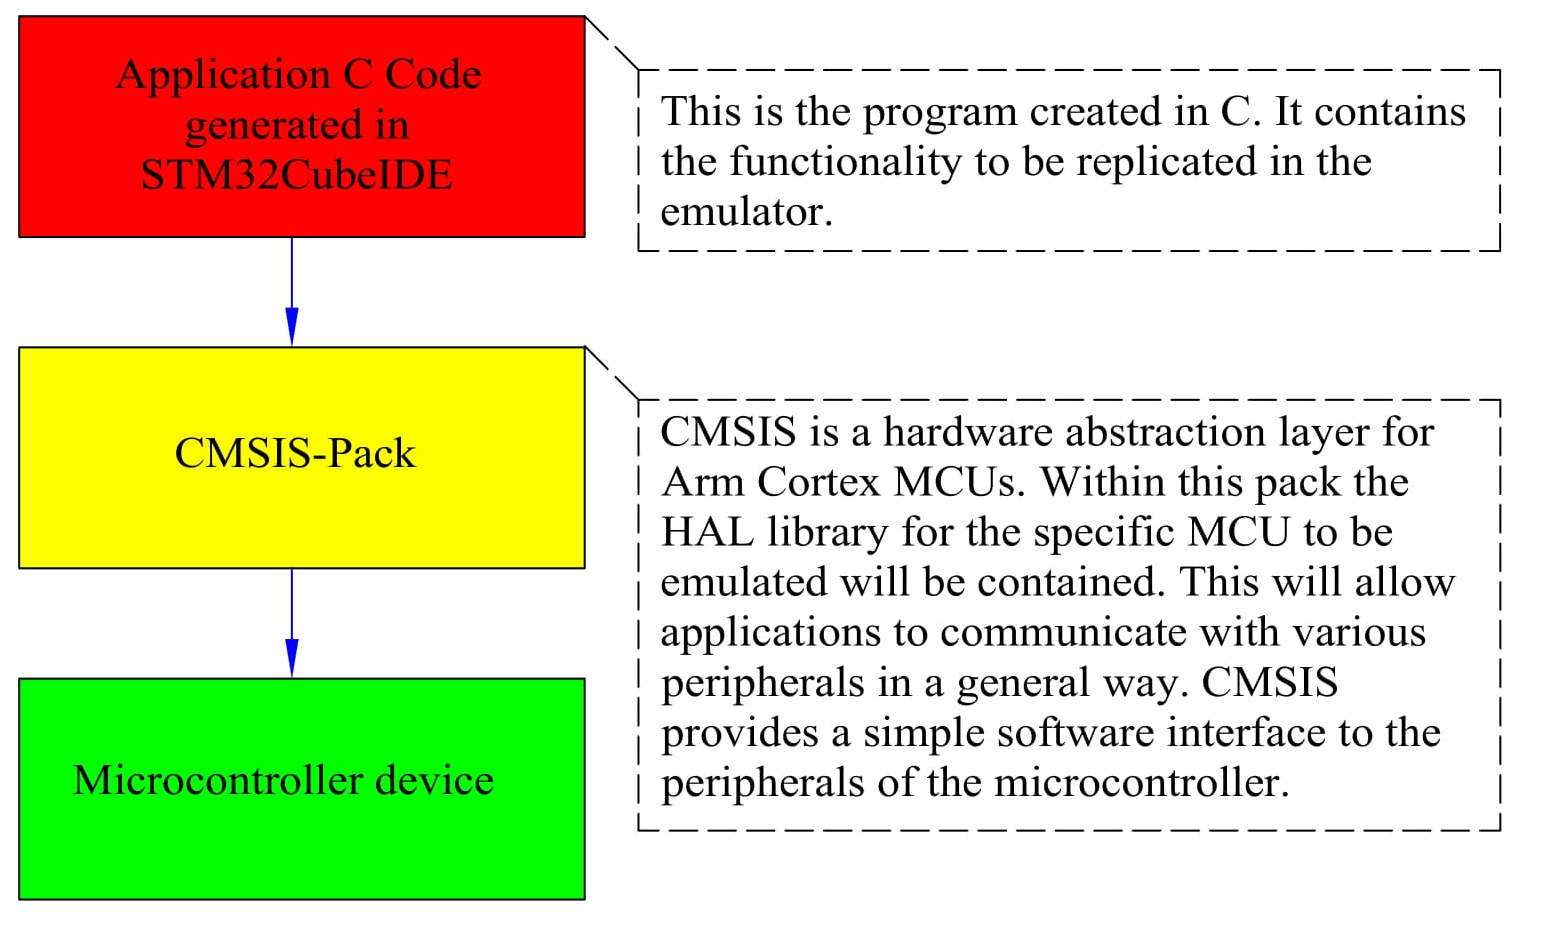
\includegraphics[width = 150mm]{cmsis.jpg}
\caption{CMSIS in context}
\label{fig:cmsis.jpg}
\end{center}
\end{figure}

Figure~\ref{fig:cmsis.jpg} shows CMSIS-Packs in relation to application code and the target \hyperref[listAbr]{MCU}. It demonstrates how \hyperref[listAbr]{CMSIS} in-short, ensures compatibility between the application and the \hyperref[listAbr]{MCU}. \hyperref[listAbr]{CMSIS}-packs are installed within the Eclipse and will be elaborated upon in \textbf{\ref{eclipse} \nameref{eclipse}}. Furthermore, the installation of \hyperref[listAbr]{CMSIS}-packs will occur within the Eclipse \hyperref[listAbr]{IDE} and will subsequently be addressed in the relevant subsection.   
\subsection{Eclipse Embedded CDT}
\label{eclipse}
Once all the prerequisites have been met as mentioned in the preceding subsection, Eclipse Embedded CDT can be installed. It will serve as a software environment wherein emulation can  occurs. When set up in the right way, it will enable a visual representation of the target board via the QEMU debugger. It is recommended that the workspace preferences for Eclipse Embedded CDT be changed as per \textbf{\nameref{E}}. The first step is to download and install Eclipse Embedded CDT found at: \color{blue}\url{https://projects.eclipse.org/projects/iot.embed-cdt/downloads/}\color{black}.
\\\\
It important to set the default Arm toolchain path to the xPack GNU Arm Embedded GCC. This is the toolchain installed in \textbf{\ref{dependencies} \nameref{dependencies} -  \nameref{toolchains}}.
\begin{figure}[H]
\begin{center}
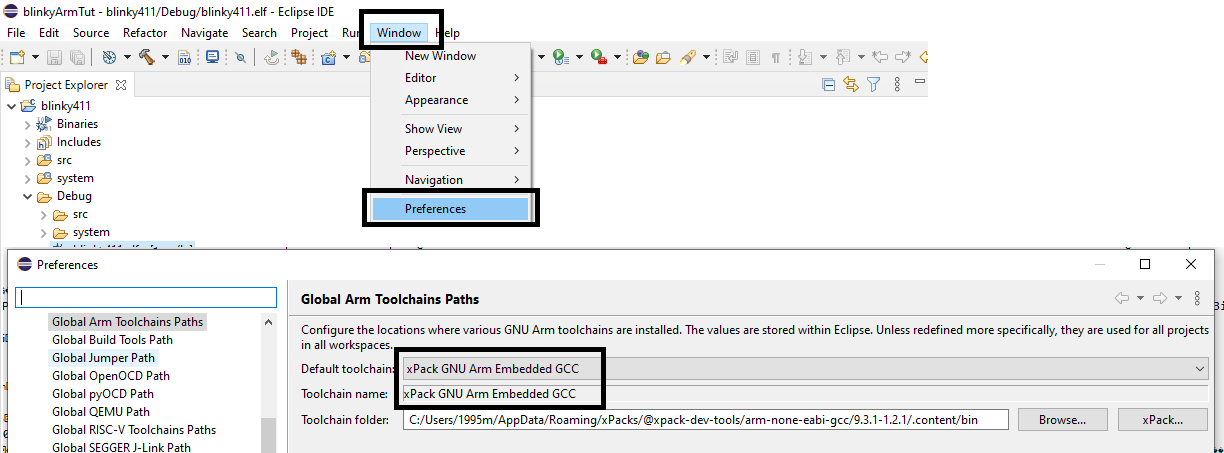
\includegraphics[width = 155mm]{pref.png}
\caption{Arm toolchains for Embedded Eclipse CDT}
\label{fig:prefArm.jpg}
\end{center}
\end{figure}

Figure~\ref{fig:prefArm.jpg} illustrates the Eclipse preferences panel. As can be seen from the figure, it is required that the default toolchain is set to xPack GNU Arm Embedded GCC. This is a required step for emulation to ultimately occur. This is in contrast to the preference settings highlighted by \textbf{\nameref{E}}, which are recommended but not necessary \cite{eclipseGuide}.

\subsection{CMSIS-packs installation}
\label{CMSISpacks}
\hyperref[listAbr]{CMSIS}-packs are described in \textbf{\ref{dependencies} \nameref{dependencies} - CMSIS Packages}. This subsection will detail their installation process within the chosen \hyperref[listAbr]{IDE}: Eclipse Embedded \hyperref[listAbr]{CDT}. It is important to note that before the CMSIS-packs are installed, a target \hyperref[listAbr]{MCU} must be specified. This is because the \hyperref[listAbr]{HAL} libraries included in the \hyperref[listAbr]{CMSIS}-packs are specific to certain \hyperref[listAbr]{MCU} families and are not completely hardware independent. It is indeed the case, that \purl{system_stm32f4xx}\hyperref[listExt]{.h} from the STM32F4 family of \hyperref[listAbr]{HAL} libraries contained in the relevent \hyperref[listAbr]{CMSIS} pack, is specific to STM32F4 \hyperref[listAbr]{MCU}s only. 
\\\\
For the purposes of addressing the problem stated in \textbf{\ref{ps} \nameref{ps}}, it thus becomes necessary to specify a target \hyperref[listAbr]{MCU}. Whilst the \hyperref[listAbr]{CMSIS}-packs and subsequent header files contained in the \hyperref[listAbr]{HAL} libraries are needed for the build process, they are not needed for emulation. It can be seen from \textbf{\ref{xpack} \nameref{xpack}}, that very few \hyperref[listAbr]{MCU}s are, in fact, available for complete emulation. The consequence of this observation is that the \hyperref[listAbr]{CMSIS}-pack designated for installation, will be dependent on the real-world \hyperref[listAbr]{MCU} and not the emulated \hyperref[listAbr]{MCU}!
\\\\
It is mentioned in \textbf{\ref{xpack} \nameref{xpack}}, that amongst the faculties most commonly used \hyperref[listAbr]{MCU}s the STM32F411VE can be found. This particular \hyperref[listAbr]{MCU} is therefore chosen as the real-world MCU to be mimicked. The \hyperref[listAbr]{CMSIS}-packs for this \hyperref[listAbr]{MCU} will thus be downloaded as indicated:

\begin{figure}[H]
\begin{center}
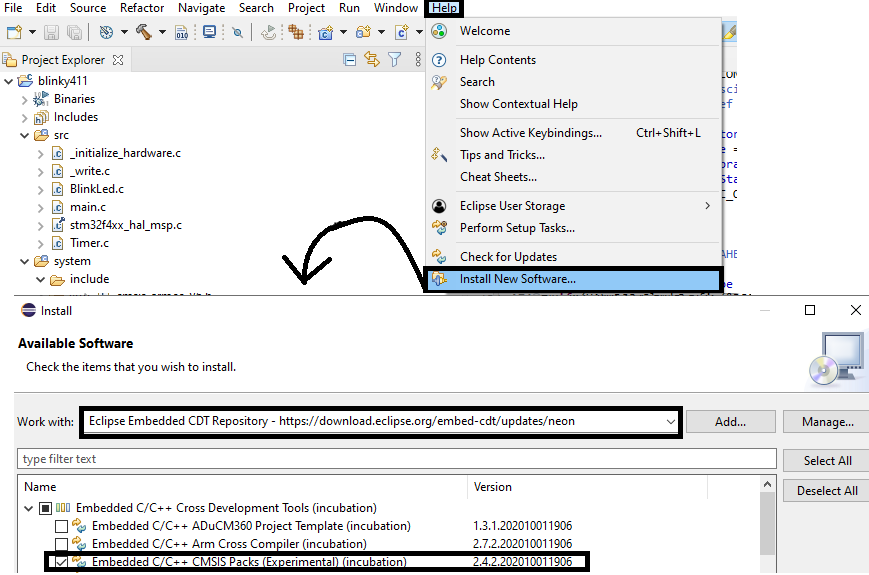
\includegraphics[width = 155mm]{cmsis1.png}
\caption{CMSIS packs download}
\label{CMSIS1}
\end{center}
\end{figure}

Once the \hyperref[listAbr]{CMSIS}-packs have been downloaded as per Figure~\ref{CMSIS1}, the specific library for the real-world \hyperref[listAbr]{MCU} can be selected and locally installed in Eclipse as follows:

\begin{figure}[H]
\begin{center}
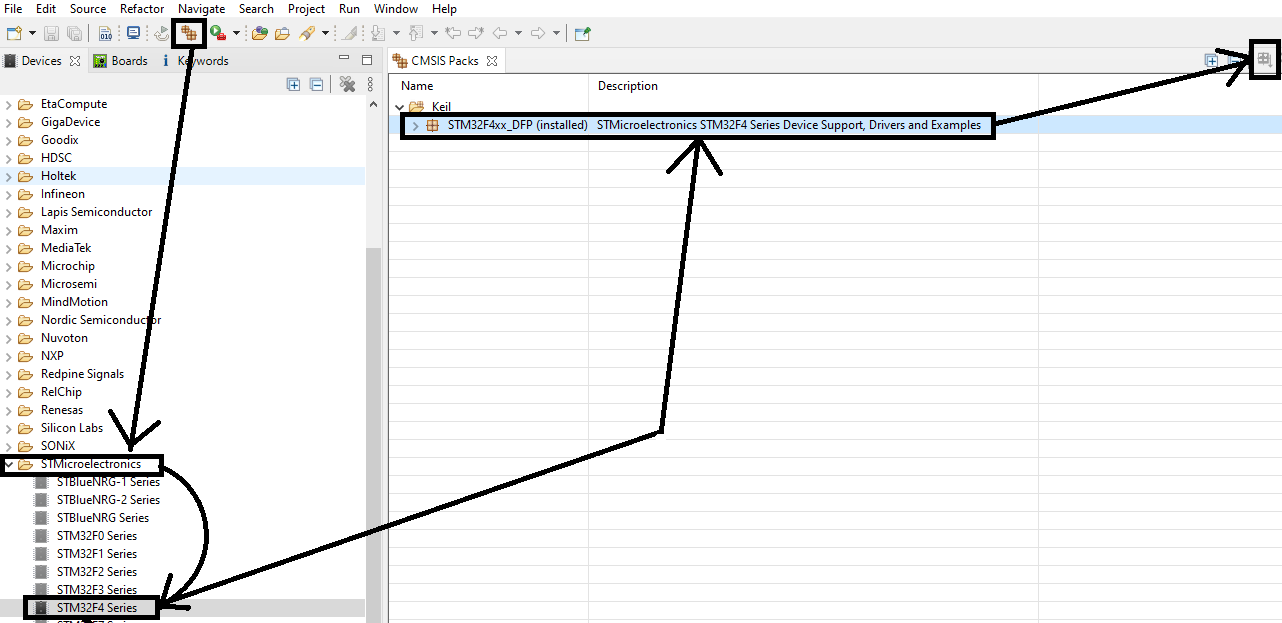
\includegraphics[scale = 0.5, angle = 90]{cmsis2.png}
\caption{CMSIS packs local install}
\label{CMSIS1}
\end{center}
\end{figure}

Once this step has been completed, emulation can take place. This is discussed in \textbf{\nameref{results}}. 










